% ============================================================
% ============================================================
% NACA0012 -- CONVECTIVE HEAT TRANSFER
% ============================================================
% ============================================================

\section[HTC]{\textbf{Convective Heat Transfer}}


% ============================================================
% NACA0012 -- Convective Heat Transfer Evaluation
% ============================================================

\begin{frame}[shrink=15]{\small NACA0012 -- Convective Heat Transfer Evaluation}
\scriptsize

\centering

\begin{minipage}{0.90\textwidth}
\begin{block}{\scriptsize Integrated Convective Heat Transfer}
The convective heat transfer is evaluated along the surface slice as
\[
\boxed{
Q_c'
=
\int
HTC(s)
\left[
T_s(s)-T_{\mathrm{rec}}(s)
\right]\,ds
}
\qquad
[Q_c'] = \mathrm{W/m}.
\]

The submitted $HTC$, surface temperature $T_s$, and pressure coefficient $C_p$
are used directly.
\end{block}
\end{minipage}

\vspace{0.15cm}

\begin{minipage}{0.90\textwidth}
\begin{block}{\scriptsize Recovery Temperature Reconstruction}
Since $T_{\mathrm{rec}}$ is not directly available from the submissions, it is
reconstructed from the submitted $C_p$ distribution:
\[
\boxed{
C_p(s)
\;\longrightarrow\;
p_e(s)
\;\longrightarrow\;
M_e(s)
\;\longrightarrow\;
T_e(s)
\;\longrightarrow\;
T_{\mathrm{rec}}(s)
}
\]

Assuming $p_s \simeq p_e$ and an isentropic external flow,
\[
\frac{p_e}{p_\infty}
=
1+\frac{\gamma}{2}M_\infty^2 C_p.
\]
\end{block}
\end{minipage}

\vspace{0.15cm}

\begin{minipage}{0.90\textwidth}
\begin{block}{\scriptsize Recovery Model}
For a turbulent boundary layer,
\[
T_{\mathrm{rec}}
=
T_e
\left[
1+r\frac{\gamma-1}{2}M_e^2
\right],
\qquad
r=Pr^{1/3}\approx0.9.
\]
\end{block}
\end{minipage}

\end{frame}


% ============================================================
% NACA0012 -- Convective Heat-Transfer Distributions
% ============================================================

\begin{frame}[shrink]{\small NACA0012 -- Convective Heat-Transfer Distributions (L1)}
\scriptsize

\begin{columns}[T,onlytextwidth]

\begin{column}{0.50\textwidth}
    \centering
    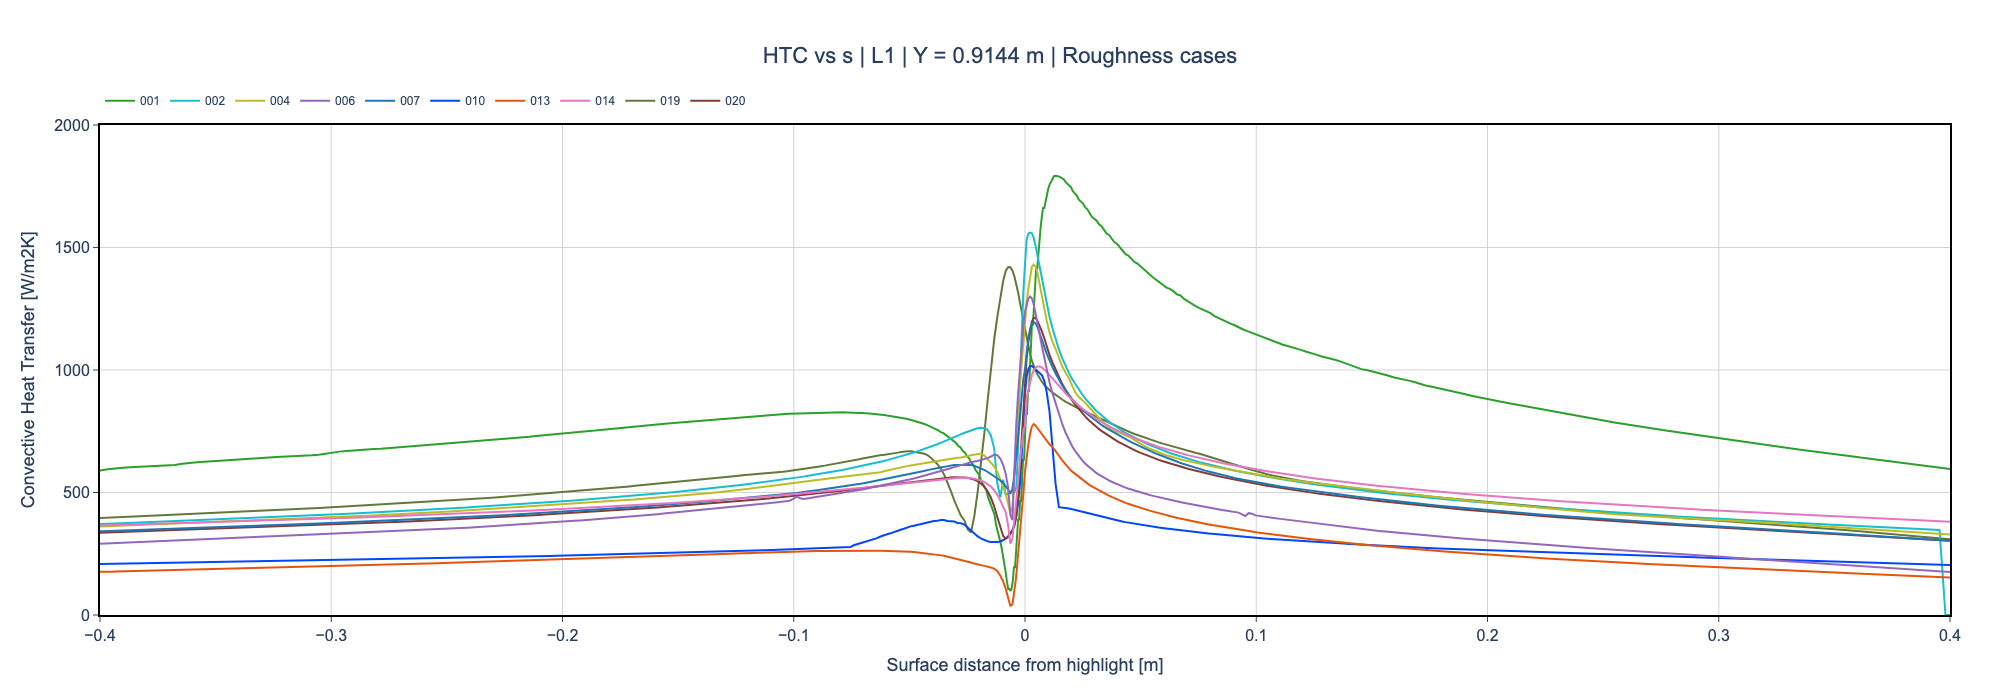
\includegraphics[width=\textwidth]{FIGURES/HTC/tc_naca0012_ae3932_L1_htc_vs_s_slice_0p9144_all_roughness.png}

    \vspace{0.05cm}

    {\scriptsize\textbf{Convective heat-transfer coefficient}}
\end{column}

\begin{column}{0.50\textwidth}
    \centering
    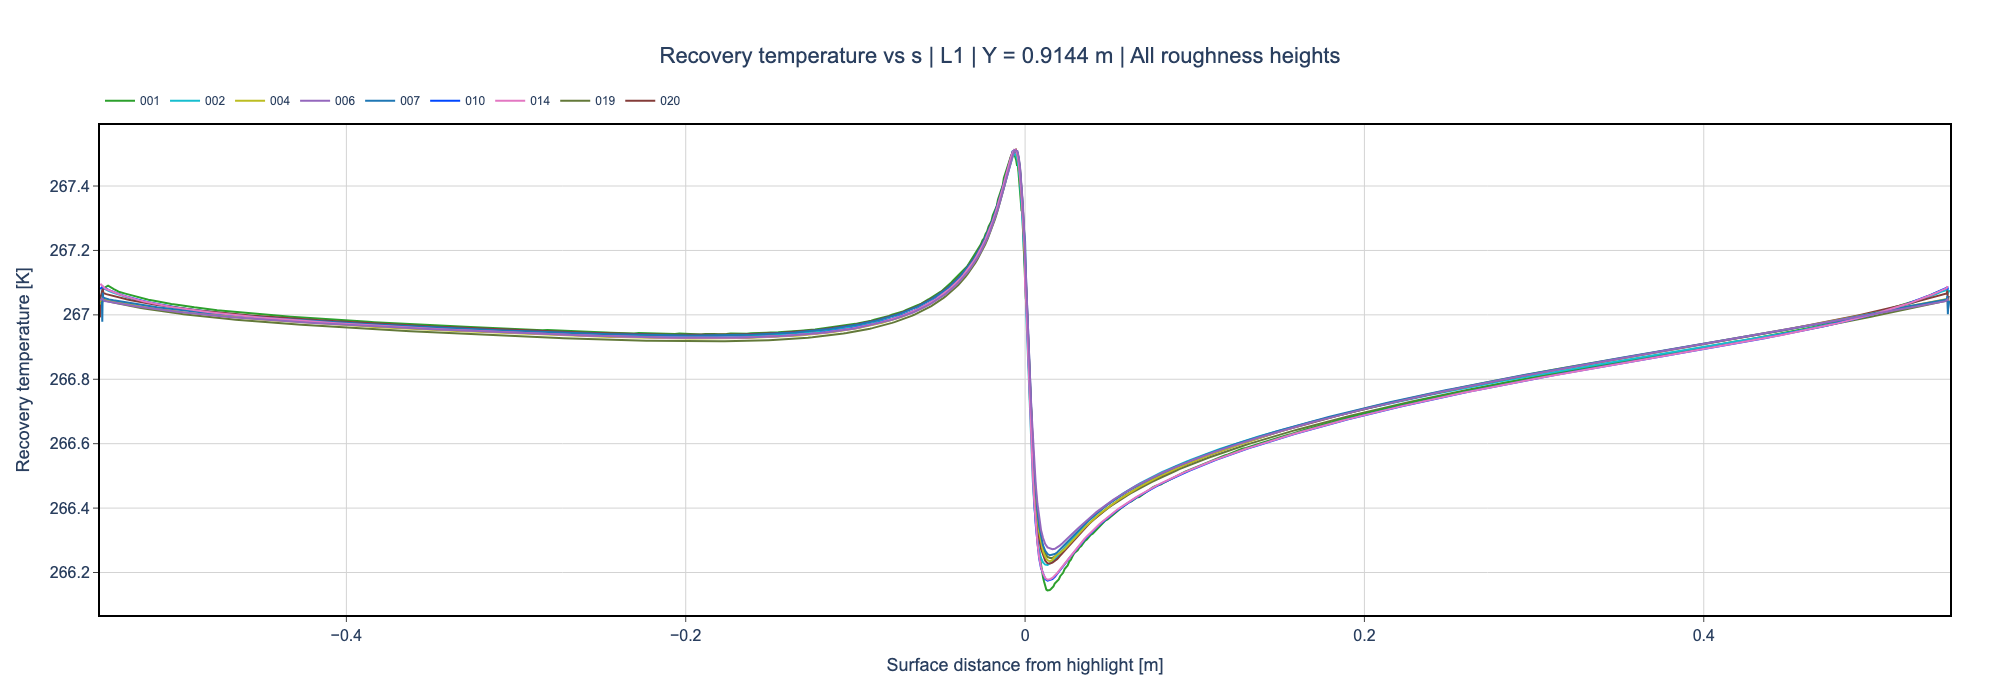
\includegraphics[width=\textwidth]{FIGURES/HTC/tc_naca0012_ae3932_L1_recovery_temperature_vs_s_slice_0p9144_all_roughness.png}

    \vspace{0.05cm}

    {\scriptsize\textbf{Reconstructed recovery temperature}}
\end{column}

\end{columns}

\vspace{0.15cm}

\begin{block}{\scriptsize Assessment}
\begin{itemize}
    \item On the L1 grid, reconstructed recovery-temperature distributions are closely clustered across submissions.
    \item Considerably larger code-to-code differences are observed in $HTC$, particularly near the leading edge.
    \item The L1 comparison indicates that the variability in the convective thermal boundary condition is primarily associated with $HTC$ rather than $T_{\mathrm{rec}}$.
    \item Differences in prescribed surface roughness should be considered when interpreting the remaining $HTC$ variability.
\end{itemize}
\end{block}

\end{frame}


% ============================================================
% NACA0012 -- Convective Heat Transfer Grid Convergence
% ============================================================

\begin{frame}{\small NACA0012 -- Convective Heat Transfer Grid Convergence}
\scriptsize

{\centering
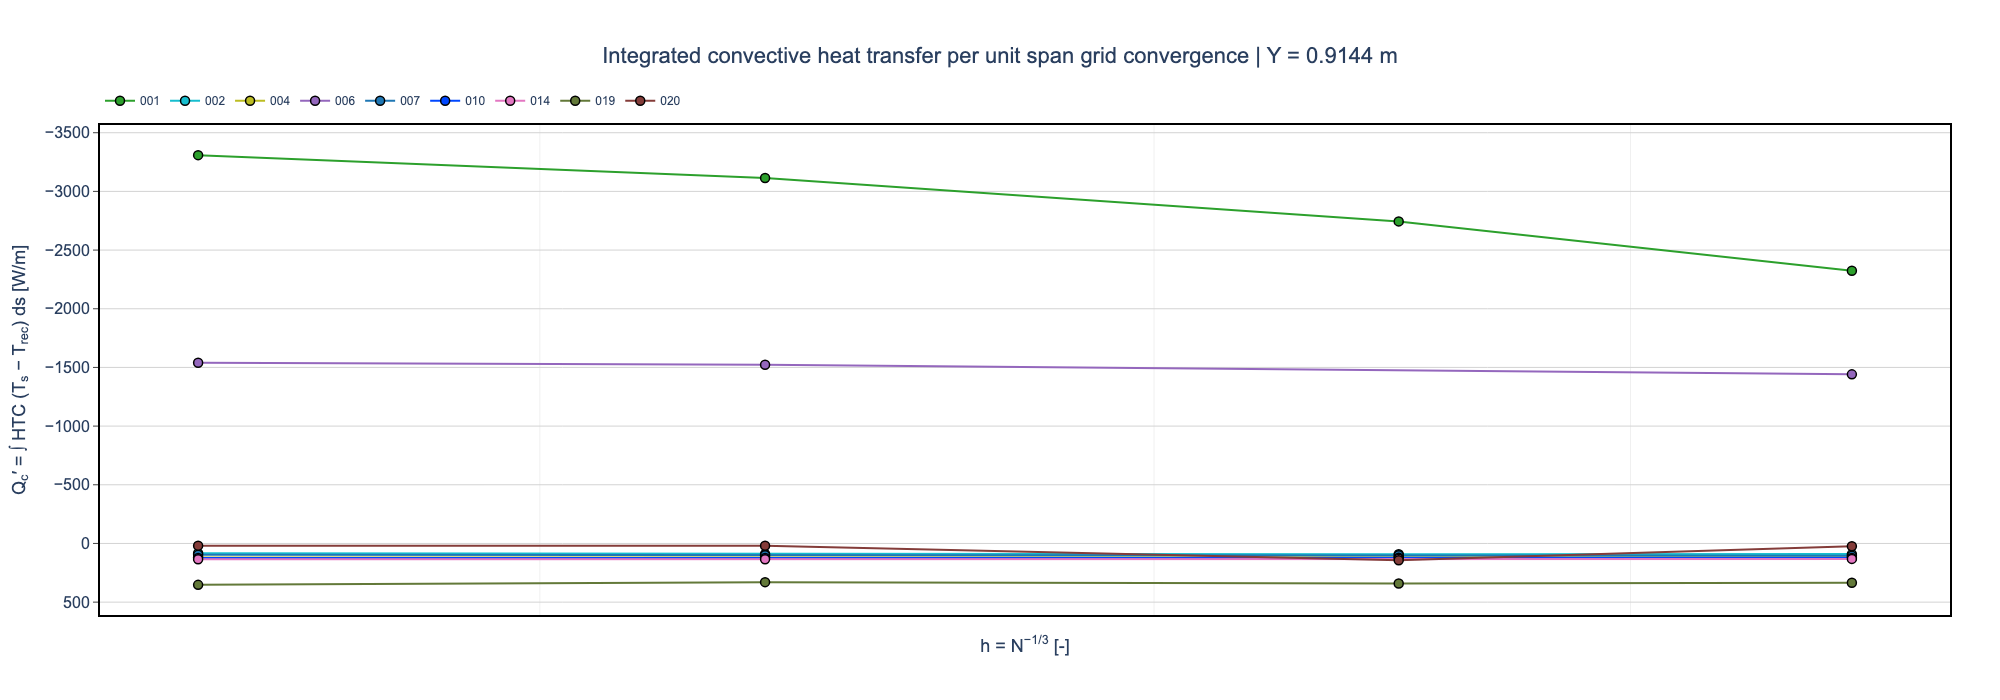
\includegraphics[width=1.0\textwidth]{FIGURES/HTC/tc_naca0012_ae3932_qc_prime_vs_n_y_0.9144.png}
\par}

\vspace{0.15cm}

\begin{block}{\scriptsize Assessment}
\begin{itemize}
    \item For most submissions, the integrated convective heat transfer exhibits relatively limited variation with spatial grid refinement.
    \item Code-to-code variability is substantially larger than the grid-refinement effect.
    \item The observed spread is primarily associated with differences in the submitted $HTC$ distributions rather than the reconstructed recovery temperature.
    \item A small number of submissions exhibit markedly different integrated heat-transfer behavior and should be distinguished from the main cluster.
\end{itemize}
\end{block}

\end{frame}


% ============================================================
% ============================================================
% END -- NACA0012 CONVECTIVE HEAT TRANSFER
% ============================================================
% ============================================================
